\ifx \allfiles \undefined
\documentclass{article}
\usepackage{booktabs}
\usepackage{multirow}
\usepackage{graphicx}
\usepackage{subfigure}

\begin{document}
\title{Discuss}
\maketitle \else \fi

\section{Discussion}\label{sec:discussion}
During our labeling process, we find several interesting results reflected by our algorithms. We distributed top 100 users of UCLA category returned by different algorithms and into several categories and described as follows.


However, the dataset for this classification problem has two disadvantages. One disadvantage is the class is unbalanced. The fraction of positive training samples is too small, which makes the learning particularly difficult. The other disadvantage is the number of features is very large, which is due to the diversity of words people used in their tweets and frequent appearance of typos and hyphen marks.


\subsection{User classification}
The users are classified into $6$ categories manually, they are active users with related bio, tweets or photos (ActiveUCLA); inactive users belongs to UCLA (InactiveUCLA); inactive users not belongs to UCLA (Inactive); user intent miss match (Intent); and user not belongs to UCLA (Negative). The classification result is in Figure \ref{fig:userclass}.

\begin{figure}[h]
\centering
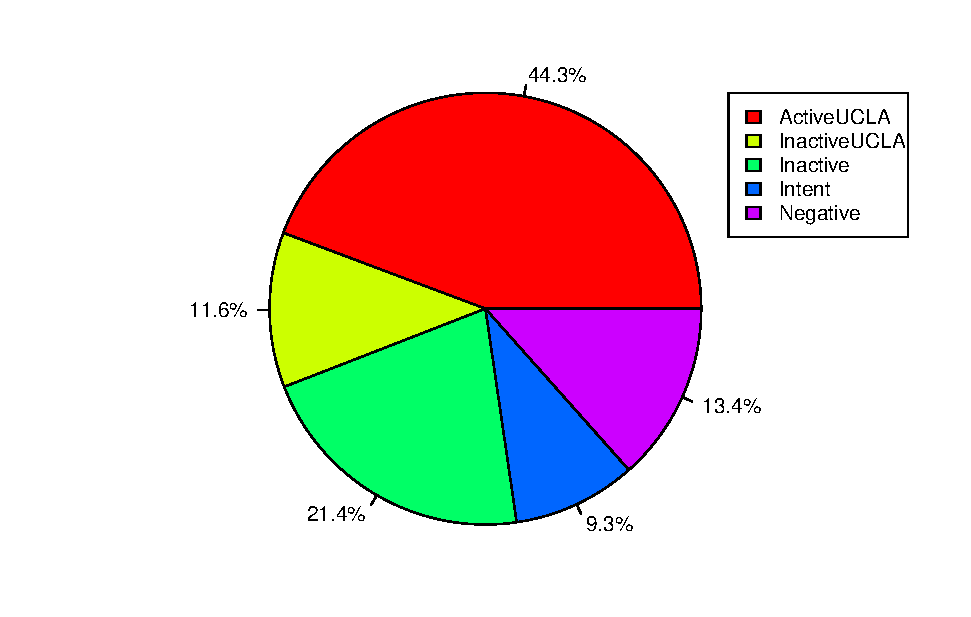
\includegraphics[width=0.5\textwidth]{experiment/uc.eps}
\caption{Manually user classification result.}
\label{fig:userclass}
\end{figure}

For active users, it is easy to see whether the user has related tweets about UCLA or photos about UCLA. For users without new tweets in recent two months, we call them inactive users and classify them according to Google result. We type their name with UCLA and see whether there is related search results.

\subsection{Intent mismatch}
The intent mismatch, labeled as ``Intent'' in Figure \ref{fig:userclass}, refers to the situations where the users are somehow related to UCLA but it is actually not belong to UCLA. The data show that intent mismatch often arises when a user follows a lot of UCLA users or a user talks about something that mentions UCLA.

There are several examples of intent mismatch. First, users may follow UCLA members in order to have more business opportunities, such as ``WeTutorLA'' and ``bombaybite''. The former one follows lot of students from UCLA, USC, UCSD and so on to let them noticed. The latter one follows a lot of organizations of UCLA because it is a restaurant near UCLA. Second, some users keeps follow back a lot of users, such as ``0neNiteStan''. This kind of users have a lot of tweets for advertisement. Third, users like ``USCTrojansNews'', ``openwestwood'' would ranked at higher position in our result. These users' tweets have significant intersection with users from UCLA. For example, ``USCTrojansNews'' often publish tweets that compare UCLA with USC while some users in UCLA category also like to do that. This makes our model make mistakes during the training process.

These kinds of intent mismatch contribute to $9.3\%$ discrepancies in the data. Typically, intent mismatch are very hard to be corrected since it requires human understanding of why this user may related to UCLA but not belongs to UCLA.

\subsection{Precision of active user}


\ifx \allfiles \undefined
\end{document}
\fi 